\documentclass{article}

\usepackage[english]{babel}
\usepackage[utf8]{inputenc}
\usepackage{amsmath,amssymb}
\usepackage{parskip}
\usepackage{graphicx}
\usepackage{subfig}
\usepackage{titling}
\usepackage{float}
% Margins
\usepackage[top=2.54cm, left=2.54cm, right=2.54cm, bottom=2.54cm,textheight=11pt]{geometry}

\predate{}
\postdate{}
\title{\vspace{-1.8cm}\textbf{Monte Carlo Simulation}}
\author{Nikhil Thota}
\date{}

\begin{document}
\maketitle

\section{Method and Results}

When the set of differential equations were solved simultaneously with the initial conditions of x(0) = y(0) = z(0) = 1 from t=0 to t=40 with a step size of 0.01. The time series plots of x,y and z vs t produced are shown below :

\vspace{-0.6cm}

\begin{figure}[h]
    \centering
    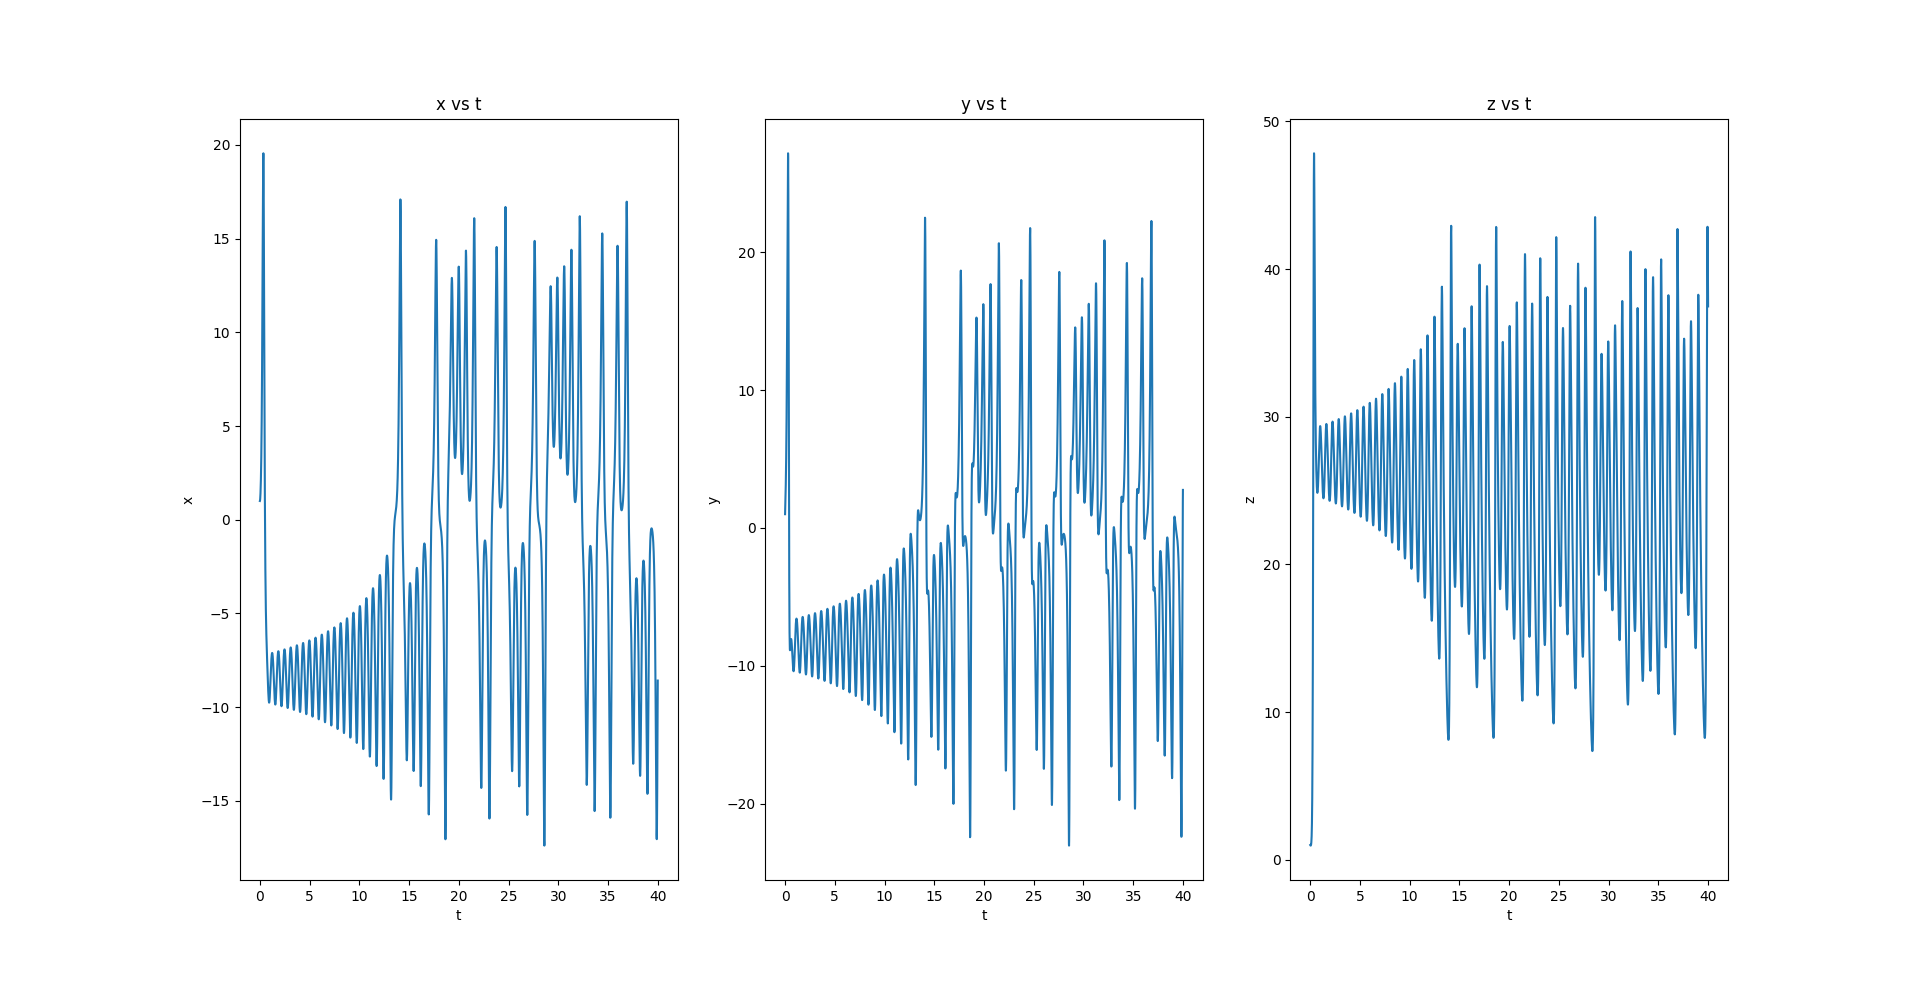
\includegraphics[width=0.5\paperwidth]{x_y_z_t.png}
    \caption{Time series plot of x, y and z till t = 40}
    \label{fig:time series plot of x,y and z}
\end{figure}

\vspace{-0.5cm}

In the next part of the problem the intial conditions are not known but are sampled from a multivariate gaussian distribution centered about (1,1,1) and having covariance of an identity matrix. 

10000 datapoints were sampled from this distribution and the set of simultaneous differential equations were solved with each of these data points as initial conditions. When the pairwise joint pdf was plotted at a few time steps beautiful plots were generated as shown below :

\vspace{-0.5cm}

\begin{figure}[H]
    \centering
    \subfloat{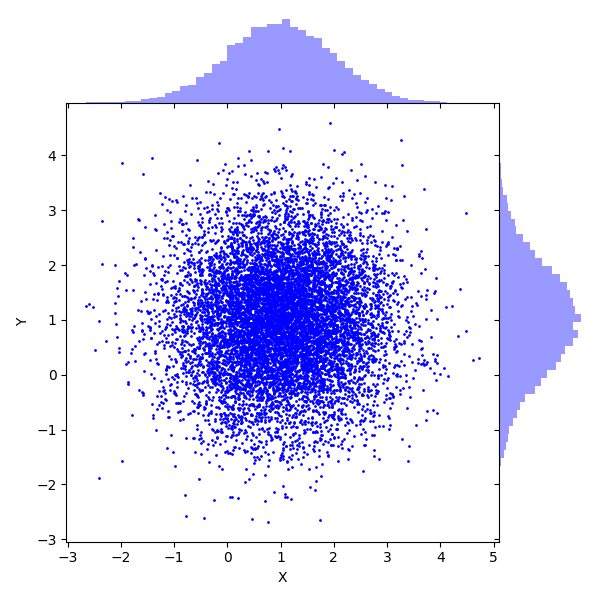
\includegraphics[width=4.3cm]{XY_0.png}}
    \subfloat{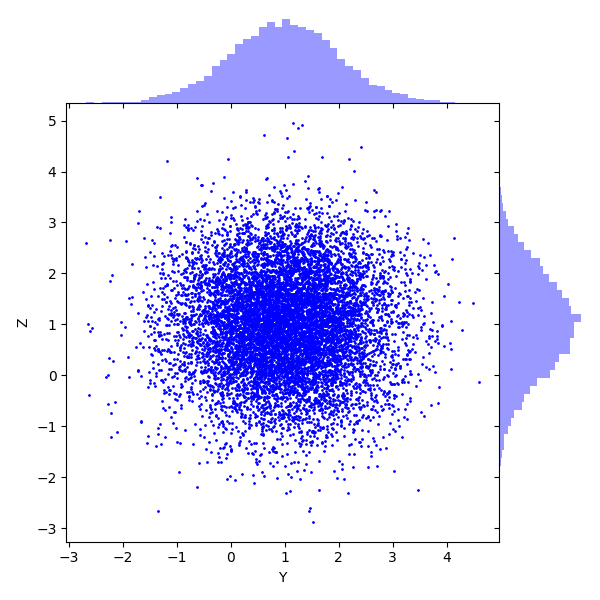
\includegraphics[width=4.3cm]{YZ_0.png}}
    \subfloat{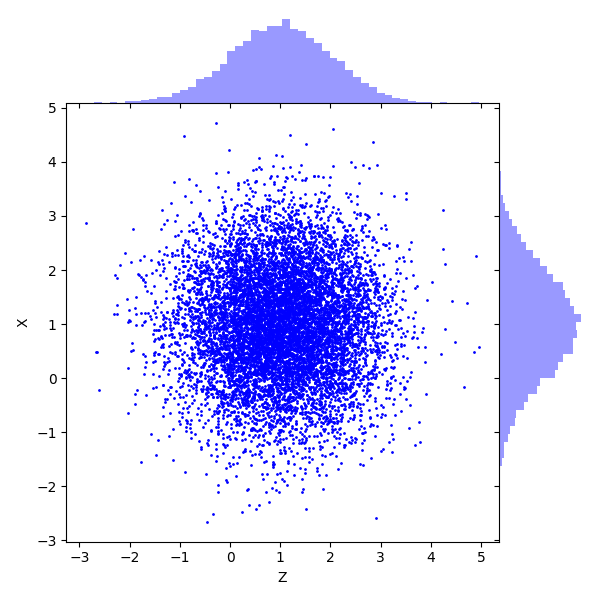
\includegraphics[width=4.3cm]{ZX_0.png}}
    \caption{At t=0 the pairwise joint pdf of x,y and z}
	\vspace{-0.4cm}
    \centering
    \subfloat{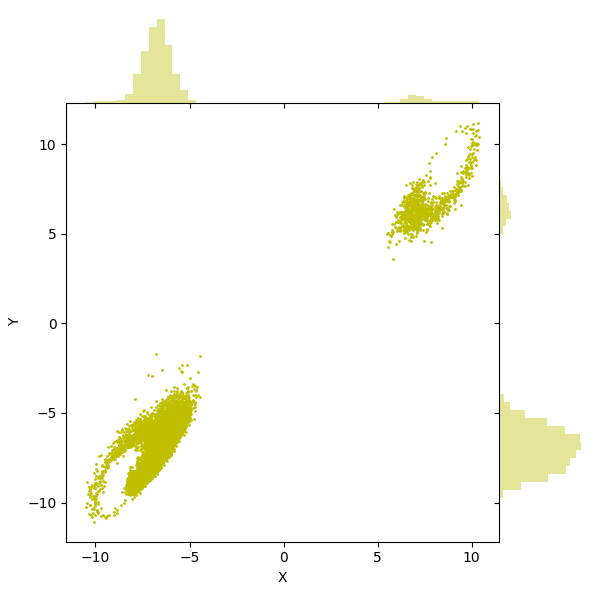
\includegraphics[width=4.3cm]{XY_5.png}}
    \subfloat{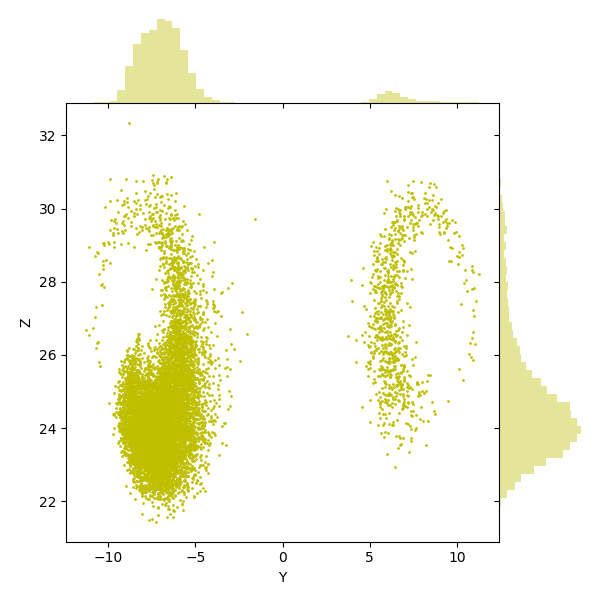
\includegraphics[width=4.3cm]{YZ_5.png}}
    \subfloat{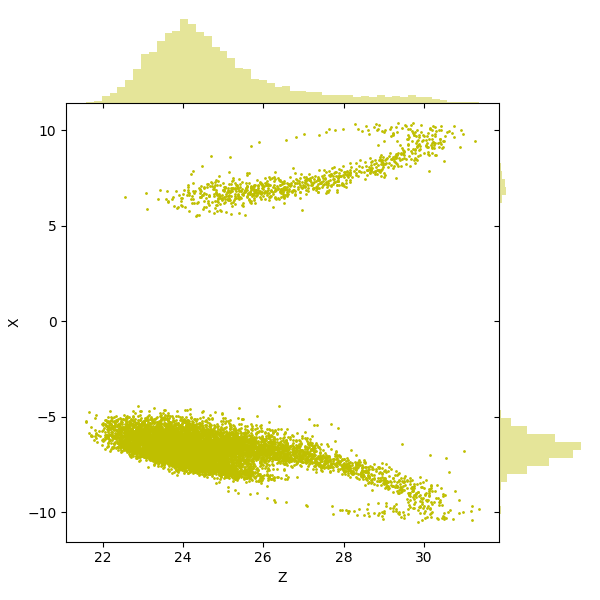
\includegraphics[width=4.3cm]{ZX_5.png}}
    \caption{At t=5 the pairwise joint pdf of x,y and z}
\end{figure}

\begin{figure}[H]
    \centering
    \subfloat{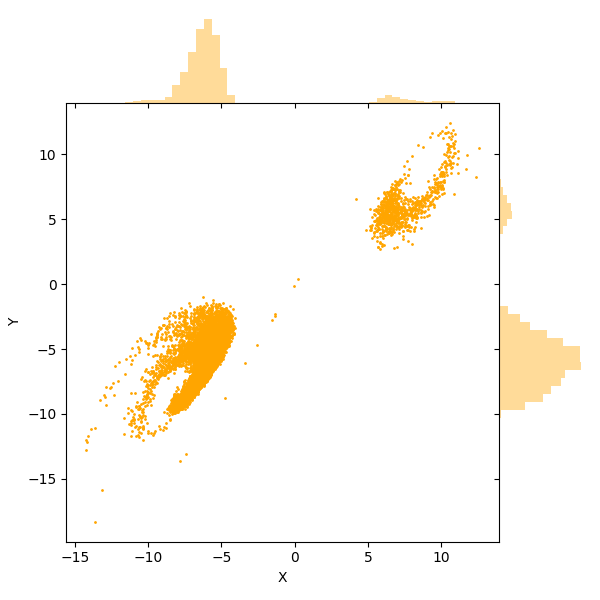
\includegraphics[width=4.3cm]{XY_7_5.png}}
    \subfloat{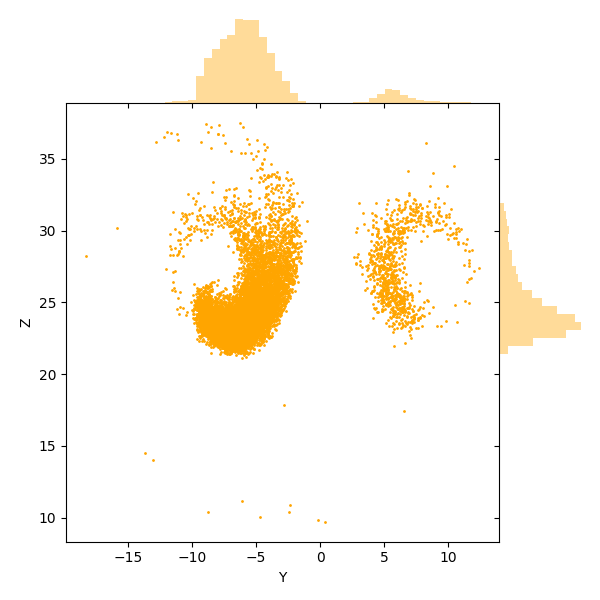
\includegraphics[width=4.3cm]{YZ_7_5.png}}
    \subfloat{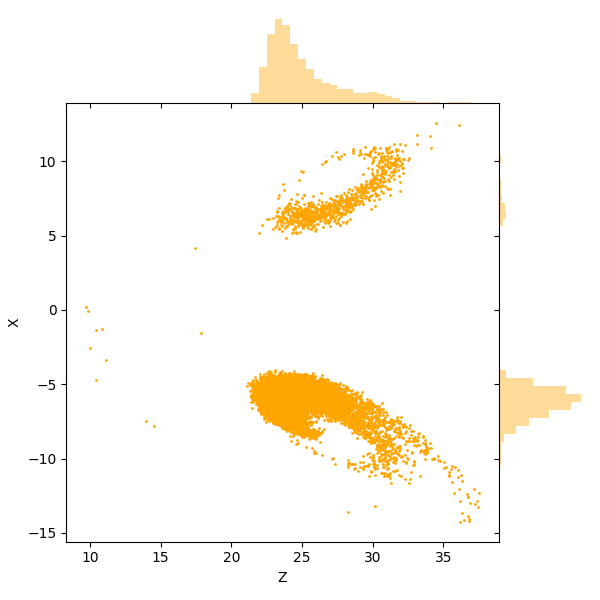
\includegraphics[width=4.3cm]{ZX_7_5.png}}
    \caption{At t=7.5 the pairwise joint pdf of x,y and z}
	\vspace{-0.4cm}
    \centering
    \subfloat{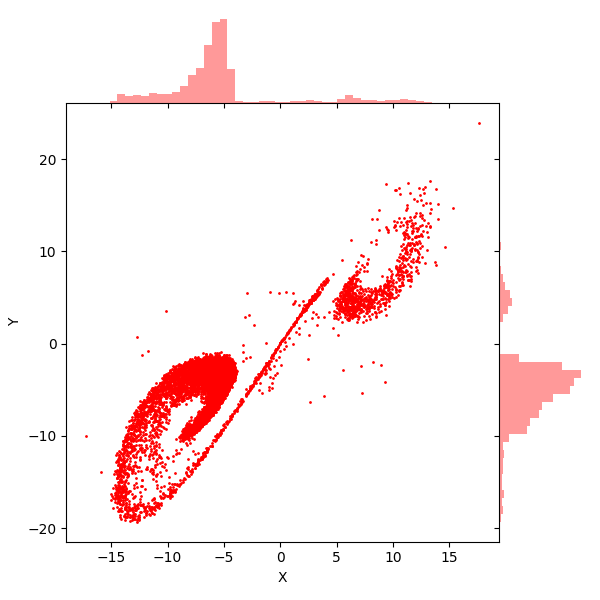
\includegraphics[width=4.3cm]{XY_10.png}}
    \subfloat{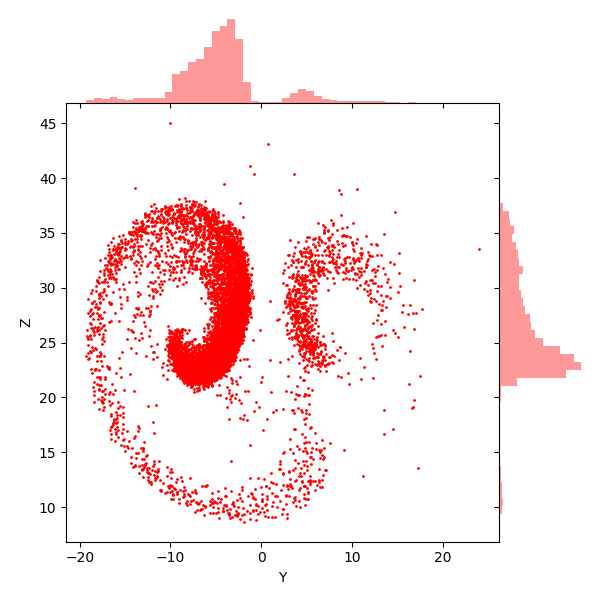
\includegraphics[width=4.3cm]{YZ_10.png}}
    \subfloat{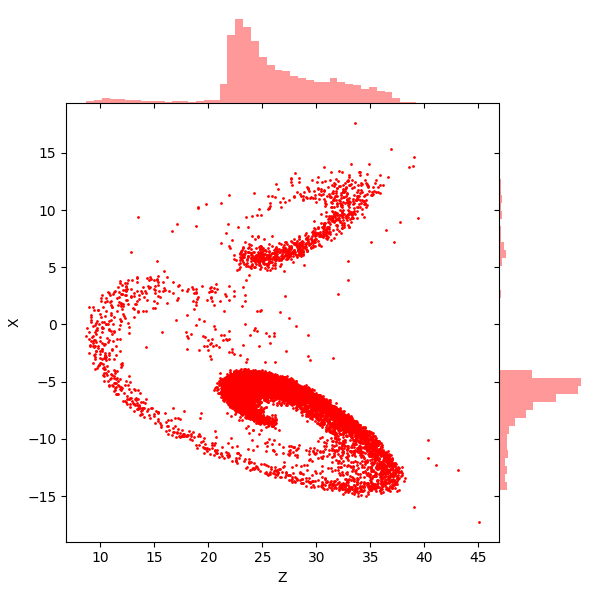
\includegraphics[width=4.3cm]{ZX_10.png}}
    \caption{At t=10 the pairwise joint pdf of x,y and z}
\end{figure}

\vspace{-0.5cm}

The pair wise joint pdf plot of x,y and z at t=0 shows the distribution of the initial conditions.

The nature of these joint pdf plots can be attributed to the oscillating nature of the time series plots of x, y and z. In the time series plots of x and y we can see that the oscillations are periodic as they shift from oscillating about a value in the positive region to oscillating about a value in the negative region and vice-versa. Whereas in the time series plot of z the oscillations occur completely in the positive region and at a higher absolute value than compared to x and y. An important point to note is that this behaviour holds true even when the initial conditions have changed from x(0)=y(0)=z(0)=1. 

The time series plot of x and y are quite similar (as seen from Figure 1) which is why the joint pdf plot x-y lies along x=y axis. Looking at the joint pdf plots of z-x and y-z we can see a heart shaped plot. The two halves of the heart are symmetric due to oscillations in the positive and negative regions of the time series plots of x and y. If all 10,000 x,y,z datapoints are plotted as a 3-D plot at each instance of time, then the xy joint pdf plot would be the 2-D projection of the view along the +z axis onto the xy plane. Similarly the yz joint pdf plot would be the 2-D projection of the view along the +x axis onto yz plane and the zx joint pdf wold be the 2-D projection of the view along the +y axis onto the zx plane.

\emph{Note 1 : The python program was written using Python 3.6.9 and was run from the terminal in Ubuntu OS.}

\end{document}